\documentclass[conference]{IEEEtran}
\IEEEoverridecommandlockouts
\usepackage[T1]{fontenc}
\usepackage{cite}
\usepackage{amsmath,amssymb}
\usepackage{graphicx}
\usepackage{booktabs}
\usepackage{url}
\usepackage{xcolor}
\usepackage{tikz}
\usetikzlibrary{positioning,arrows.meta,shapes.geometric}

% ---------------------------------------------------------------------------
% Every benchmark number below is produced by scripts/make_paper_tables.py
% from the raw run logs and pasted between the GENERATED RESULTS markers.
% To update: regenerate generated_results.tex and replace that block.
% ---------------------------------------------------------------------------
\newcommand{\rs}{Rs.\,}
% centred second row of authors in the IEEE author block
\makeatletter
\newcommand{\linebreakand}{\end{@IEEEauthorhalign}\hfill\mbox{}\par\mbox{}\hfill\begin{@IEEEauthorhalign}}
\makeatother
\newcommand{\res}[1]{\ifcsname res@#1\endcsname\csname res@#1\endcsname\else\textbf{??}\fi}
% ===== BEGIN GENERATED RESULTS (scripts/make_paper_tables.py, run 2026-09-27_1546, complete) =====
% AUTO-GENERATED by scripts/make_paper_tables.py - do not edit by hand.
% Source run: 2026-09-27_1546; complete=True
\makeatletter
\expandafter\def\csname res@T1-B_tool-acc\endcsname{100.0}
\expandafter\def\csname res@T1-B_tool-lo\endcsname{72.2}
\expandafter\def\csname res@T1-B_tool-hi\endcsname{100.0}
\expandafter\def\csname res@T1-B_tool-noans\endcsname{0.0}
\expandafter\def\csname res@T1-B_tool-medlat\endcsname{0.120}
\expandafter\def\csname res@T1-B_tool-meanlat\endcsname{0.254}
\expandafter\def\csname res@T1-B_tool-p95lat\endcsname{1.413}
\expandafter\def\csname res@T1-B_tool-tok\endcsname{0}
\expandafter\def\csname res@T1-B_tool-medtok\endcsname{0}
\expandafter\def\csname res@T1-B_tool-n\endcsname{10}
\expandafter\def\csname res@T1-B_tool-k\endcsname{10}
\expandafter\def\csname res@T1-B_tool-cons\endcsname{10}
\expandafter\def\csname res@T1-B_tool-cases\endcsname{10}
\expandafter\def\csname res@T1-B_tool-maxtok\endcsname{0}
\expandafter\def\csname res@T1-B_tool-trunc\endcsname{0}
\expandafter\def\csname res@T1-B_tool-miss\endcsname{0}
\expandafter\def\csname res@T1-B_tool-wrong\endcsname{0}
\expandafter\def\csname res@T1-B_tool-nofinal\endcsname{0}
\expandafter\def\csname res@T1-A_deployed-acc\endcsname{96.7}
\expandafter\def\csname res@T1-A_deployed-lo\endcsname{83.3}
\expandafter\def\csname res@T1-A_deployed-hi\endcsname{99.4}
\expandafter\def\csname res@T1-A_deployed-noans\endcsname{3.3}
\expandafter\def\csname res@T1-A_deployed-medlat\endcsname{1,644.4}
\expandafter\def\csname res@T1-A_deployed-meanlat\endcsname{2,289.9}
\expandafter\def\csname res@T1-A_deployed-p95lat\endcsname{3,823.6}
\expandafter\def\csname res@T1-A_deployed-tok\endcsname{2,694}
\expandafter\def\csname res@T1-A_deployed-medtok\endcsname{2,636}
\expandafter\def\csname res@T1-A_deployed-n\endcsname{30}
\expandafter\def\csname res@T1-A_deployed-k\endcsname{29}
\expandafter\def\csname res@T1-A_deployed-cons\endcsname{9}
\expandafter\def\csname res@T1-A_deployed-cases\endcsname{10}
\expandafter\def\csname res@T1-A_deployed-maxtok\endcsname{3,396}
\expandafter\def\csname res@T1-A_deployed-trunc\endcsname{0}
\expandafter\def\csname res@T1-A_deployed-miss\endcsname{1}
\expandafter\def\csname res@T1-A_deployed-wrong\endcsname{0}
\expandafter\def\csname res@T1-A_deployed-nofinal\endcsname{1}
\expandafter\def\csname res@T1-A_direct-acc\endcsname{100.0}
\expandafter\def\csname res@T1-A_direct-lo\endcsname{88.6}
\expandafter\def\csname res@T1-A_direct-hi\endcsname{100.0}
\expandafter\def\csname res@T1-A_direct-noans\endcsname{0.0}
\expandafter\def\csname res@T1-A_direct-medlat\endcsname{2,481.5}
\expandafter\def\csname res@T1-A_direct-meanlat\endcsname{4,299.2}
\expandafter\def\csname res@T1-A_direct-p95lat\endcsname{7,297.8}
\expandafter\def\csname res@T1-A_direct-tok\endcsname{1,421}
\expandafter\def\csname res@T1-A_direct-medtok\endcsname{1,116}
\expandafter\def\csname res@T1-A_direct-n\endcsname{30}
\expandafter\def\csname res@T1-A_direct-k\endcsname{30}
\expandafter\def\csname res@T1-A_direct-cons\endcsname{10}
\expandafter\def\csname res@T1-A_direct-cases\endcsname{10}
\expandafter\def\csname res@T1-A_direct-maxtok\endcsname{3,489}
\expandafter\def\csname res@T1-A_direct-trunc\endcsname{0}
\expandafter\def\csname res@T1-A_direct-miss\endcsname{0}
\expandafter\def\csname res@T1-A_direct-wrong\endcsname{0}
\expandafter\def\csname res@T1-A_direct-nofinal\endcsname{0}
\expandafter\def\csname res@T1-route\endcsname{10/10}
\expandafter\def\csname res@T2-B_tool-acc\endcsname{100.0}
\expandafter\def\csname res@T2-B_tool-lo\endcsname{75.7}
\expandafter\def\csname res@T2-B_tool-hi\endcsname{100.0}
\expandafter\def\csname res@T2-B_tool-noans\endcsname{0.0}
\expandafter\def\csname res@T2-B_tool-medlat\endcsname{0.855}
\expandafter\def\csname res@T2-B_tool-meanlat\endcsname{0.985}
\expandafter\def\csname res@T2-B_tool-p95lat\endcsname{2.488}
\expandafter\def\csname res@T2-B_tool-tok\endcsname{0}
\expandafter\def\csname res@T2-B_tool-medtok\endcsname{0}
\expandafter\def\csname res@T2-B_tool-n\endcsname{12}
\expandafter\def\csname res@T2-B_tool-k\endcsname{12}
\expandafter\def\csname res@T2-B_tool-cons\endcsname{12}
\expandafter\def\csname res@T2-B_tool-cases\endcsname{12}
\expandafter\def\csname res@T2-B_tool-maxtok\endcsname{0}
\expandafter\def\csname res@T2-B_tool-trunc\endcsname{0}
\expandafter\def\csname res@T2-B_tool-miss\endcsname{0}
\expandafter\def\csname res@T2-B_tool-wrong\endcsname{0}
\expandafter\def\csname res@T2-B_tool-nofinal\endcsname{0}
\expandafter\def\csname res@T2-A_deployed-acc\endcsname{0.0}
\expandafter\def\csname res@T2-A_deployed-lo\endcsname{0.0}
\expandafter\def\csname res@T2-A_deployed-hi\endcsname{9.6}
\expandafter\def\csname res@T2-A_deployed-noans\endcsname{100.0}
\expandafter\def\csname res@T2-A_deployed-medlat\endcsname{1,245.9}
\expandafter\def\csname res@T2-A_deployed-meanlat\endcsname{3,128.4}
\expandafter\def\csname res@T2-A_deployed-p95lat\endcsname{7,539.7}
\expandafter\def\csname res@T2-A_deployed-tok\endcsname{2,519}
\expandafter\def\csname res@T2-A_deployed-medtok\endcsname{2,522}
\expandafter\def\csname res@T2-A_deployed-n\endcsname{36}
\expandafter\def\csname res@T2-A_deployed-k\endcsname{0}
\expandafter\def\csname res@T2-A_deployed-cons\endcsname{12}
\expandafter\def\csname res@T2-A_deployed-cases\endcsname{12}
\expandafter\def\csname res@T2-A_deployed-maxtok\endcsname{2,576}
\expandafter\def\csname res@T2-A_deployed-trunc\endcsname{0}
\expandafter\def\csname res@T2-A_deployed-miss\endcsname{36}
\expandafter\def\csname res@T2-A_deployed-wrong\endcsname{0}
\expandafter\def\csname res@T2-A_deployed-nofinal\endcsname{36}
\expandafter\def\csname res@T2-A_direct-acc\endcsname{58.3}
\expandafter\def\csname res@T2-A_direct-lo\endcsname{42.2}
\expandafter\def\csname res@T2-A_direct-hi\endcsname{72.9}
\expandafter\def\csname res@T2-A_direct-noans\endcsname{38.9}
\expandafter\def\csname res@T2-A_direct-medlat\endcsname{8,236.9}
\expandafter\def\csname res@T2-A_direct-meanlat\endcsname{7,630.1}
\expandafter\def\csname res@T2-A_direct-p95lat\endcsname{14,683.4}
\expandafter\def\csname res@T2-A_direct-tok\endcsname{3,882}
\expandafter\def\csname res@T2-A_direct-medtok\endcsname{4,425}
\expandafter\def\csname res@T2-A_direct-n\endcsname{36}
\expandafter\def\csname res@T2-A_direct-k\endcsname{21}
\expandafter\def\csname res@T2-A_direct-cons\endcsname{6}
\expandafter\def\csname res@T2-A_direct-cases\endcsname{12}
\expandafter\def\csname res@T2-A_direct-maxtok\endcsname{5,087}
\expandafter\def\csname res@T2-A_direct-trunc\endcsname{14}
\expandafter\def\csname res@T2-A_direct-miss\endcsname{15}
\expandafter\def\csname res@T2-A_direct-wrong\endcsname{1}
\expandafter\def\csname res@T2-A_direct-nofinal\endcsname{14}
\expandafter\def\csname res@T2-route\endcsname{12/12}
\expandafter\def\csname res@T3-B_tool-acc\endcsname{100.0}
\expandafter\def\csname res@T3-B_tool-lo\endcsname{51.0}
\expandafter\def\csname res@T3-B_tool-hi\endcsname{100.0}
\expandafter\def\csname res@T3-B_tool-noans\endcsname{0.0}
\expandafter\def\csname res@T3-B_tool-medlat\endcsname{3.298}
\expandafter\def\csname res@T3-B_tool-meanlat\endcsname{3.570}
\expandafter\def\csname res@T3-B_tool-p95lat\endcsname{5.055}
\expandafter\def\csname res@T3-B_tool-tok\endcsname{0}
\expandafter\def\csname res@T3-B_tool-medtok\endcsname{0}
\expandafter\def\csname res@T3-B_tool-n\endcsname{4}
\expandafter\def\csname res@T3-B_tool-k\endcsname{4}
\expandafter\def\csname res@T3-B_tool-cons\endcsname{4}
\expandafter\def\csname res@T3-B_tool-cases\endcsname{4}
\expandafter\def\csname res@T3-B_tool-maxtok\endcsname{0}
\expandafter\def\csname res@T3-B_tool-trunc\endcsname{0}
\expandafter\def\csname res@T3-B_tool-miss\endcsname{0}
\expandafter\def\csname res@T3-B_tool-wrong\endcsname{0}
\expandafter\def\csname res@T3-B_tool-nofinal\endcsname{0}
\expandafter\def\csname res@T3-A_deployed-acc\endcsname{0.0}
\expandafter\def\csname res@T3-A_deployed-lo\endcsname{0.0}
\expandafter\def\csname res@T3-A_deployed-hi\endcsname{24.3}
\expandafter\def\csname res@T3-A_deployed-noans\endcsname{91.7}
\expandafter\def\csname res@T3-A_deployed-medlat\endcsname{1,917.8}
\expandafter\def\csname res@T3-A_deployed-meanlat\endcsname{3,396.8}
\expandafter\def\csname res@T3-A_deployed-p95lat\endcsname{18,553.2}
\expandafter\def\csname res@T3-A_deployed-tok\endcsname{2,285}
\expandafter\def\csname res@T3-A_deployed-medtok\endcsname{2,282}
\expandafter\def\csname res@T3-A_deployed-n\endcsname{12}
\expandafter\def\csname res@T3-A_deployed-k\endcsname{0}
\expandafter\def\csname res@T3-A_deployed-cons\endcsname{3}
\expandafter\def\csname res@T3-A_deployed-cases\endcsname{4}
\expandafter\def\csname res@T3-A_deployed-maxtok\endcsname{2,324}
\expandafter\def\csname res@T3-A_deployed-trunc\endcsname{0}
\expandafter\def\csname res@T3-A_deployed-miss\endcsname{12}
\expandafter\def\csname res@T3-A_deployed-wrong\endcsname{1}
\expandafter\def\csname res@T3-A_deployed-nofinal\endcsname{11}
\expandafter\def\csname res@T3-A_direct-acc\endcsname{25.0}
\expandafter\def\csname res@T3-A_direct-lo\endcsname{8.9}
\expandafter\def\csname res@T3-A_direct-hi\endcsname{53.2}
\expandafter\def\csname res@T3-A_direct-noans\endcsname{75.0}
\expandafter\def\csname res@T3-A_direct-medlat\endcsname{9,715.3}
\expandafter\def\csname res@T3-A_direct-meanlat\endcsname{8,970.1}
\expandafter\def\csname res@T3-A_direct-p95lat\endcsname{13,575.9}
\expandafter\def\csname res@T3-A_direct-tok\endcsname{4,867}
\expandafter\def\csname res@T3-A_direct-medtok\endcsname{5,693}
\expandafter\def\csname res@T3-A_direct-n\endcsname{12}
\expandafter\def\csname res@T3-A_direct-k\endcsname{3}
\expandafter\def\csname res@T3-A_direct-cons\endcsname{4}
\expandafter\def\csname res@T3-A_direct-cases\endcsname{4}
\expandafter\def\csname res@T3-A_direct-maxtok\endcsname{5,697}
\expandafter\def\csname res@T3-A_direct-trunc\endcsname{9}
\expandafter\def\csname res@T3-A_direct-miss\endcsname{9}
\expandafter\def\csname res@T3-A_direct-wrong\endcsname{0}
\expandafter\def\csname res@T3-A_direct-nofinal\endcsname{9}
\expandafter\def\csname res@T3-route\endcsname{4/4}
\expandafter\def\csname res@ALL-B_tool-k\endcsname{26}
\expandafter\def\csname res@ALL-B_tool-n\endcsname{26}
\expandafter\def\csname res@ALL-A_deployed-k\endcsname{29}
\expandafter\def\csname res@ALL-A_deployed-n\endcsname{78}
\expandafter\def\csname res@ALL-A_direct-k\endcsname{54}
\expandafter\def\csname res@ALL-A_direct-n\endcsname{78}
\expandafter\def\csname res@NODATA-n\endcsname{48}
\expandafter\def\csname res@NODATA-nofinal\endcsname{47}
\expandafter\def\csname res@NODATA-valued\endcsname{1}
\expandafter\def\csname res@infra\endcsname{2}
\expandafter\def\csname res@fetch-med\endcsname{261}
\expandafter\def\csname res@fetch-p95\endcsname{4,859}
\expandafter\def\csname res@model\endcsname{openai/gpt-oss-120b}
\expandafter\def\csname res@repeats\endcsname{3}
\expandafter\def\csname res@X-chatgpt-gpt5.6-luna-1\endcsname{10/10}
\expandafter\def\csname res@X-chatgpt-gpt5.6-luna-2\endcsname{9/12}
\expandafter\def\csname res@X-chatgpt-gpt5.6-luna-3\endcsname{4/4}
\expandafter\def\csname res@X-chatgpt-gpt5.6-luna-all\endcsname{23/26}
\expandafter\def\csname res@X-claude-sonnet5-low-1\endcsname{10/10}
\expandafter\def\csname res@X-claude-sonnet5-low-2\endcsname{12/12}
\expandafter\def\csname res@X-claude-sonnet5-low-3\endcsname{4/4}
\expandafter\def\csname res@X-claude-sonnet5-low-all\endcsname{26/26}
\makeatother
\def\RunComplete{1}

\newcommand{\MainResultsTable}{%
\begin{table*}[t]\centering
\caption{Accuracy, cost and latency by task tier and system arm. Accuracy is exact agreement with the independent reference within tolerance; 95\% Wilson intervals in brackets. Latency is wall-clock per answer; tokens are LLM tokens per answer (prompt + completion, including hidden reasoning).}
\label{tab:main}\small\resizebox{\textwidth}{!}{%
\begin{tabular}{llrrrrrr}\toprule
Tier & Arm & $n$ & Exact acc.\ (\%) [95\% CI] & No answer (\%) & Median lat.\ (ms) & p95 lat.\ (ms) & Mean tokens \\ \midrule
Portfolio arithmetic & Foleo tools (ours) & 10 & 100.0 [72.2, 100.0] & 0.0 & 0.120 & 1.413 & 0 \\
 & Groq + full data & 30 & 100.0 [88.6, 100.0] & 0.0 & 2,481.5 & 7,297.8 & 1,421 \\
 & Groq chatbot (no prices) & 30 & 96.7 [83.3, 99.4] & 3.3 & 1,644.4 & 3,823.6 & 2,694 \\
\midrule
Stock time-series metrics & Foleo tools (ours) & 12 & 100.0 [75.7, 100.0] & 0.0 & 0.855 & 2.488 & 0 \\
 & Groq + full data & 36 & 58.3 [42.2, 72.9] & 38.9 & 8,236.9 & 14,683.4 & 3,882 \\
 & Groq chatbot (no prices) & 36 & 0.0 [0.0, 9.6] & 100.0 & 1,245.9 & 7,539.7 & 2,519 \\
\midrule
Portfolio risk metrics & Foleo tools (ours) & 4 & 100.0 [51.0, 100.0] & 0.0 & 3.298 & 5.055 & 0 \\
 & Groq + full data & 12 & 25.0 [8.9, 53.2] & 75.0 & 9,715.3 & 13,575.9 & 4,867 \\
 & Groq chatbot (no prices) & 12 & 0.0 [0.0, 24.3] & 91.7 & 1,917.8 & 18,553.2 & 2,285 \\
\bottomrule\end{tabular}}\end{table*}}

\newcommand{\PerCaseTable}{%
\begin{table*}[t]\centering
\caption{Per-case answers on the time-series tiers (all repeats). ``--'' = no final numeric answer.}
\label{tab:percase}\scriptsize
\begin{tabular}{lrlll}\toprule
Case & Reference & Foleo tools & Groq + full data & Groq chatbot (no prices) \\ \midrule
RELIANCE.NS:total\_return & -6.99 & -6.99 & -6.99, -6.99, -6.99 & --, --, -- \\
RELIANCE.NS:max\_drawdown & -8.66 & -8.66 & -8.66, -8.66, -8.65 & --, --, -- \\
RELIANCE.NS:var95 & 1.69 & 1.69 & --, --, -- & --, --, -- \\
RELIANCE.NS:rsi14 & 25.66 & 25.66 & 25.65, --, -- & --, --, -- \\
TCS.NS:total\_return & -0.61 & -0.61 & -0.61, -0.61, -0.61 & --, --, -- \\
TCS.NS:max\_drawdown & -15.83 & -15.83 & --, -15.85, -15.84 & --, --, -- \\
TCS.NS:var95 & 2.75 & 2.75 & --, --, -- & --, --, -- \\
TCS.NS:rsi14 & 22.21 & 22.21 & 22.22, --, 22.22 & --, --, -- \\
HDFCBANK.NS:total\_return & -7.62 & -7.62 & -7.62, -7.62, -7.62 & --, --, -- \\
HDFCBANK.NS:max\_drawdown & -17.2 & -17.2 & --, -17.2, -17.2 & --, --, -- \\
HDFCBANK.NS:var95 & 2.19 & 2.19 & --, --, -- & --, --, -- \\
HDFCBANK.NS:rsi14 & 61.4 & 61.4 & 61.38, 62.68, 61.4 & --, --, -- \\
portfolio:sharpe & -4.2766 & -4.2766 & --, --, -- & --, --, -- \\
portfolio:var95 & 2.38 & 2.38 & --, --, -- & --, --, -- \\
portfolio:max\_drawdown & -20.77 & -20.77 & --, --, -- & --, --, -- \\
portfolio:total\_return & -19.27 & -19.27 & -19.27, -19.27, -19.27 & -6.74, --, -- \\
\bottomrule\end{tabular}\end{table*}}

\newcommand{\ExternalTable}{%
\begin{table}[t]\centering
\caption{External assistants on the identical prompt pack (single session, built-in code execution used by both). Exact answers / prompts.}
\label{tab:external}\small
\begin{tabular}{lrrrr}\toprule
Assistant & Tier 1 & Tier 2 & Tier 3 & Total \\ \midrule
ChatGPT (GPT-5.6 Luna) & 10/10 & 9/12 & 4/4 & 23/26 \\
Claude Sonnet 5 (low) & 10/10 & 12/12 & 4/4 & 26/26 \\
\bottomrule\end{tabular}\end{table}}
% ===== END GENERATED RESULTS =====

\begin{document}

% ============================== COVER PAGE ==================================
\begin{titlepage}
\begin{center}
 \vspace*{2.5cm}  % adjust the number as you like

	Capstone Project Report on\\
	\null
	\textbf{\large \textbf{FOLEO}}\\
	\null

	by \\
	\textbf{Shrey Golekar (231DS031)}
	\\\textbf{Sanchit Srisha Udupa (231IT060)}
	\\\textbf{Prasanna Kumar (231MN010)}\\
	\vspace{0.8em}
	\large{\textit{under the guidance of}} \\
	\vspace{0.8em}

	\large{\textbf{Dr. Shrutilipi Bhattacharjee}}\\
	\vspace{1.2em}
	\IfFileExists{symbol.jpg}{
\includegraphics[width=6cm, height=6cm]{symbol.jpg}}{%
	  \fbox{\parbox[c][6cm][c]{6cm}{\centering\small Upload the NITK logo\\as \texttt{symbol.jpg}}}}\\
	\vspace{1.2em}
DEPARTMENT OF INFORMATION TECHNOLOGY\\
NATIONAL INSTITUTE OF TECHNOLOGY KARNATAKA\\
SURATHKAL, MANGALORE - 575025\\
\null
September, 2026\\
\end{center}
\end{titlepage}

% ================================ PAPER =====================================
\title{Foleo: Deterministic Tool Grounding for Reliable LLM-Based Portfolio Analytics}

\author{
\IEEEauthorblockN{Shrey Golekar}
\IEEEauthorblockA{\textit{Department of Computational and Data Sciences}\\
\textit{NIT-Surathkal}\\
Surathkal, Mangalore, India\\
shreygolekar.231ds031@nitk.edu.in}
\and
\IEEEauthorblockN{Sanchit Srisha Udupa}
\IEEEauthorblockA{\textit{Department of Information Technology}\\
\textit{NIT-Surathkal}\\
Surathkal, Mangalore, India\\
sanchit.231it060@nitk.edu.in}
\linebreakand
\IEEEauthorblockN{Prasanna Kumar}
\IEEEauthorblockA{\textit{Department of Mining Engineering}\\
\textit{NIT-Surathkal}\\
Surathkal, Mangalore, India\\
cprasannakumar.231mn010@nitk.edu.in}
\and
\IEEEauthorblockN{Shrutilipi Bhattacharjee}
\IEEEauthorblockA{\textit{Department of Information Technology}\\
\textit{NIT-Surathkal}\\
Surathkal, Mangalore, India\\
shrutilipi@nitk.edu.in}
}

\maketitle

\ifnum\RunComplete=0
\begin{center}\fcolorbox{red}{white}{\parbox{0.92\columnwidth}{\centering\small\color{red}
DRAFT: the benchmark run is incomplete. Values marked \textbf{??} or taken from a partial run must be
regenerated before submission.}}\end{center}
\fi

\begin{abstract}
Large language models (LLMs) are increasingly used as conversational front-ends for personal investing, yet
portfolio questions demand exact arithmetic and precisely defined risk metrics. This paper presents Foleo, a
broker-integrated portfolio assistant in which an LLM handles dialogue while a deterministic tool layer computes
every quantitative answer. Foleo maps broker holdings (Zerodha, Upstox) to exchange tickers, routes numeric
requests---including implicit portfolio-level requests such as ``what is my Sharpe ratio?''---to 16 tested
functions, and answers them without invoking the LLM. We evaluate the design with a three-tier benchmark
(portfolio arithmetic, single-stock time-series metrics, and portfolio risk metrics) on National Stock Exchange
(NSE) prices pinned to a fixed snapshot, in which every system receives identical inputs and ground truth comes
from an independent reference implementation. Against the open-weight reasoning model gpt-oss-120b, evaluated
both as deployed in the application and with the complete data in its context, the tool path answered
\res{ALL-B_tool-k} of \res{ALL-B_tool-n} cases exactly with zero LLM tokens and a few milliseconds of computation at most.
The LLM was reliable on simple holdings arithmetic, but on time-series metrics it consumed
\res{T2-A_direct-tok} tokens per answer on average and reached \res{T2-A_direct-acc}\% exact accuracy, with every
missing answer caused by exhausting its token budget. Without price history, the deployed assistant gave no value in
\res{NODATA-nofinal} of \res{NODATA-n} requests, but once presented the portfolio's gain since purchase as its
three-month return. Two commercial assistants solved
the task pack only by writing and executing their own code, and one of them implemented a different RSI formula
than the one specified. We also document four failure modes uncovered while building the system---reasoning-budget
exhaustion, ticker mis-resolution, metric-definition drift and evaluation artefacts---together with their fixes.
\end{abstract}

\begin{IEEEkeywords}
Large Language Models, Tool-Augmented Reasoning, Financial Question Answering, Portfolio Analytics,
Numerical Reasoning, Risk Metrics, Hallucination, Evaluation Methodology.
\end{IEEEkeywords}

% ============================================================================
\section{Introduction}
Conversational assistants built on large language models (LLMs) are an attractive interface for retail
investors: a user can ask ``how is my portfolio doing?'' or ``how risky is it?'' in plain language instead of
navigating dashboards. Such questions, however, have exact answers. Invested value, profit and loss, a Sharpe
ratio or a Value-at-Risk figure is either correct or wrong, and a plausible but wrong number is worse than no
answer because it can drive a financial decision.

LLMs are known to be unreliable at exact multi-step computation. Their accuracy on compositional arithmetic decays
quickly with problem size~\cite{dziri2023faith}, and they can produce fluent statements that are not supported by
their inputs~\cite{ji2023hallucination}. Financial question-answering benchmarks confirm the gap in the domain:
models trail human experts on numerical reasoning over financial reports~\cite{chen2021finqa,zhu2021tatqa,chen2022convfinqa},
and on FinanceBench a retrieval-augmented GPT-4-Turbo answered incorrectly or refused 81\% of
questions~\cite{islam2023financebench}. A well-studied remedy is to let the model delegate computation to external
tools or generated programs~\cite{schick2023toolformer,gao2023pal,chen2023pot,yao2023react,mialon2023augmented}.

Most of this evidence comes from question-answering benchmarks rather than from deployed assistants connected to
real brokerage accounts. In a deployed system, wrong numbers arise not only from arithmetic: holdings must be
resolved to the correct securities, a metric such as RSI must be computed with one specific definition, the model
may exhaust its generation budget, and the evaluation harness itself can report spurious agreement. This paper
studies these issues end to end in Foleo, a portfolio assistant we built for Indian retail investors. Its
contributions are:
\begin{enumerate}
\item \textbf{A tool-grounded assistant architecture.} Foleo separates conversation (LLM) from computation
(deterministic tools). A rule-based router resolves broker holdings to exchange tickers, recognises implicit
portfolio-level requests, and answers them from 16 deterministic functions without an LLM call.
\item \textbf{A controlled, reproducible benchmark.} Three task tiers are posed to every system with identical
data: a pinned NSE price snapshot, explicit metric formulas, a fixed answer format and ground truth from an
independent reference implementation. Every raw response, the snapshot and the scoring code are retained in the
project repository.
\item \textbf{Empirical findings} on accuracy, token cost, latency, run-to-run consistency and behaviour under
missing data for a current open-weight reasoning model~\cite{openai2025gptoss}, complemented by two commercial
assistants.
\item \textbf{A catalogue of failure modes} found during development, each with a fix and a regression test,
including evaluation artefacts that had initially overstated the case for tools.
\end{enumerate}

% ============================================================================
\section{Related Work}
\subsection{Numerical reasoning in LLMs}
Chain-of-thought prompting improves multi-step reasoning by eliciting intermediate steps~\cite{wei2022cot}, but it
leaves the arithmetic itself to token generation. Dziri et al.~\cite{dziri2023faith} show that transformers solve
compositional tasks such as multi-digit multiplication largely by pattern matching over sub-computations, with
accuracy falling sharply as problem size grows. Hallucination---content unsupported by the source---is a
documented property of neural text generation~\cite{ji2023hallucination}.

\subsection{Tool-augmented and program-aided models}
Toolformer trains a model to call APIs, including a calculator, when helpful~\cite{schick2023toolformer}. PAL and
Program-of-Thoughts prompting have the model write a program that an interpreter executes, removing arithmetic
from generation; PoT reports gains on the financial datasets FinQA, ConvFinQA and TAT-QA~\cite{gao2023pal,chen2023pot}.
ReAct interleaves reasoning with actions~\cite{yao2023react}, and Mialon et al.~\cite{mialon2023augmented} survey
tool-augmented models. In these approaches the model still decides \emph{what} to compute; Foleo instead fixes
both the computation and the metric definition in tested code, and uses the LLM only where no tool applies.

\subsection{Financial question answering and finance LLMs}
FinQA~\cite{chen2021finqa}, TAT-QA~\cite{zhu2021tatqa} and ConvFinQA~\cite{chen2022convfinqa} evaluate numerical
reasoning over financial tables and text; FinanceBench~\cite{islam2023financebench} evaluates open-book QA over
company filings. Domain models such as BloombergGPT~\cite{wu2023bloomberggpt} improve financial language
understanding but are not designed to guarantee exact computation. Our benchmark differs in targeting
\emph{personal portfolio} analytics over broker holdings and price series, and in holding the input data
identical across all systems.

\subsection{Risk and performance metrics}
Foleo implements standard definitions: the Sharpe ratio~\cite{sharpe1994}, historical Value-at-Risk~\cite{jorion2007var}
using the linear-interpolation sample quantile~\cite{hyndman1996quantiles}, maximum drawdown~\cite{magdon2004mdd}
and the Relative Strength Index~\cite{wilder1978}. Several of these have competing variants (e.g., Wilder's
smoothed RSI versus a simple moving average of gains and losses), which is why the formula must be stated
explicitly in any comparison.

% ============================================================================
\section{System Design}
\subsection{Overview}
Foleo consists of a FastAPI back end, a React (Vite) web client and a local SQLite store. Users link Zerodha
(Kite Connect) and/or Upstox accounts through OAuth; holdings from all linked brokers are merged into one
portfolio. Market data (daily prices and fundamentals) is obtained from Yahoo Finance through the \texttt{yfinance}
library. The conversational layer uses an OpenAI-compatible chat API; the deployment evaluated here uses the
open-weight reasoning model \texttt{gpt-oss-120b}~\cite{openai2025gptoss} served by Groq.

\begin{figure}[t]
\centering
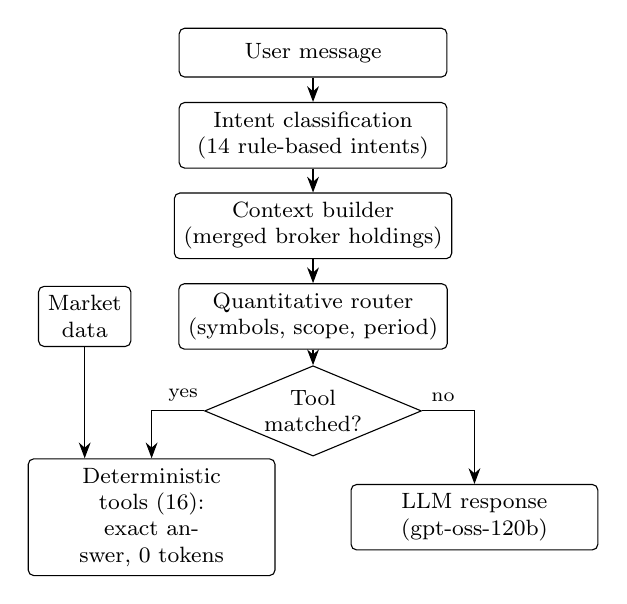
\begin{tikzpicture}[>={Stealth[length=2mm]},
  box/.style={draw, rounded corners=2pt, align=center, font=\footnotesize, minimum width=3.4cm, minimum height=0.62cm},
  sbox/.style={draw, rounded corners=2pt, align=center, font=\footnotesize, text width=2.9cm, minimum height=0.62cm},
  dec/.style={draw, diamond, aspect=2.4, align=center, font=\footnotesize, inner sep=1pt}]
\node[box] (q) at (0,0) {User message};
\node[box] (intent) at (0,-1.05) {Intent classification\\(14 rule-based intents)};
\node[box] (ctx) at (0,-2.2) {Context builder\\(merged broker holdings)};
\node[box] (route) at (0,-3.35) {Quantitative router\\(symbols, scope, period)};
\node[dec] (d) at (0,-4.55) {Tool\\matched?};
\node[sbox] (tool) at (-2.05,-5.9) {Deterministic tools (16):\\exact answer, 0 tokens};
\node[sbox] (llm) at (2.05,-5.9) {LLM response\\(gpt-oss-120b)};
\node[draw, rounded corners=2pt, align=center, font=\footnotesize] (md) at (-2.9,-3.35) {Market\\data};
\draw[->] (q) -- (intent);
\draw[->] (intent) -- (ctx);
\draw[->] (ctx) -- (route);
\draw[->] (route) -- (d);
\draw[->] (d.west) -| node[pos=0.2, above, font=\scriptsize] {yes} (tool.north);
\draw[->] (d.east) -| node[pos=0.2, above, font=\scriptsize] {no} (llm.north);
\draw[->] (md.south) -- (md.south |- tool.north);
\end{tikzpicture}
\caption{Foleo's conversational pipeline. Numeric requests that match a tool are answered deterministically;
only the remaining requests reach the LLM.}
\label{fig:pipeline}
\end{figure}

\subsection{Conversational pipeline}
Fig.~\ref{fig:pipeline} shows the request flow. A rule-based classifier assigns one of 14 intents (e.g.,
portfolio summary, risk, rebalancing, goal tracking). A context builder assembles the merged holdings and
per-holding statistics. The quantitative router then inspects the message; if it selects a tool and the tool
succeeds, Foleo returns the tool's formatted answer directly, records zero LLM tokens, and never calls the model.
Otherwise the LLM answers with the portfolio context in its prompt. If the LLM is unavailable or returns an empty
reply, a deterministic summary is returned instead of an empty message.

\subsection{Symbol resolution and portfolio scope}\label{sec:symbols}
Broker records identify a holding by trading symbol and exchange (e.g., \texttt{IDEA} on NSE), whereas the market
data source expects an exchange-qualified ticker (\texttt{IDEA.NS}). Foleo maps each holding to its ticker using the
exchange (\texttt{.NS} for NSE, \texttt{.BO} for BSE). Tokens in the user's message are treated as securities only
if they are a known alias (e.g., ``gold''), carry an exchange suffix, match a held symbol, or are written in
capitals; ordinary words such as ``portfolio'' are never treated as tickers. When a metric is requested and no
security is named, the request applies to the whole portfolio.

For portfolio scope, Foleo evaluates the current holdings over the look-back window. With $q_i$ the quantity of
holding $i$ and $P_{i,t}$ its closing price on trading day $t$ (days common to all holdings),
\begin{equation}
V_t = \sum_i q_i P_{i,t}, \qquad r_t = \frac{V_t}{V_{t-1}} - 1, \quad t = 1,\dots,T .
\end{equation}
Single-stock metrics use $V_t = P_t$. Every metric function accepts either a ticker or a precomputed series, so
stock-level and portfolio-level answers share one implementation.

\subsection{Metric definitions}
With $\bar r$ and $s_r$ the sample mean and sample standard deviation of $\{r_t\}$, Foleo computes
\begin{align}
R_{\text{total}} &= 100\,(V_T / V_0 - 1),\\
\text{MDD} &= 100 \min_{t}\Big(V_t \big/ \max_{u\le t} V_u - 1\Big),\\
\text{VaR}_{95} &= -100\,\hat Q_{0.05}(\{r_t\}),\\
\text{Sharpe} &= \frac{\bar r - r_f/252}{s_r}\sqrt{252},\quad r_f = 0.05,\\
\text{RSI}_{14} &= 100 - \frac{100}{1 + \bar G_{14}/\bar L_{14}},
\end{align}
where $\hat Q_{0.05}$ is the linear-interpolation sample quantile~\cite{hyndman1996quantiles} and $\bar G_{14}$,
$\bar L_{14}$ are the simple means of the last 14 daily close-to-close gains and losses (not Wilder's smoothed
average~\cite{wilder1978}). Beta uses sample covariance and sample variance consistently. Holdings arithmetic
uses invested value $I=\sum_i q_i a_i$ (with average buy price $a_i$), current value $C=\sum_i q_i p_i$ (with last
price $p_i$), $\text{P\&L} = C - I$ and $\text{P\&L\%} = 100(C-I)/I$. For evaluation, a transparent
classification rule maps P\&L\% to Buy ($\ge 10$), Hold ($0 < x < 10$), Trim ($-10 < x \le 0$) or Exit ($x \le -10$), where $x$ is the P\&L\%. The rule
is illustrative and is not investment advice.

\subsection{Routing and verification}
The router is an ordered table of patterns (first match wins, so ``value at risk'' is matched before the generic
``risk''), uses word boundaries so that, e.g., ``various'' does not trigger VaR, and extracts an explicit
look-back period (1 month to 5 years) when stated; otherwise each metric keeps its own default window. The
chatbot test suite (56 tests) passes, including a regression test for each failure mode in
Section~\ref{sec:failures}.

% ============================================================================
\section{Experimental Methodology}
\subsection{Research questions}
\begin{itemize}
\item \textbf{RQ1 (accuracy):} Given identical data and explicit formulas, how often does an LLM reproduce the
exact value that the deterministic tools produce?
\item \textbf{RQ2 (cost and latency):} What token and time cost does each path incur?
\item \textbf{RQ3 (missing data):} When the data needed for a metric is absent from its context, does the deployed
assistant fabricate a value or decline?
\item \textbf{RQ4 (external assistants):} Do general-purpose assistants with their own code execution match a
fixed tool layer?
\end{itemize}

\subsection{Data}
\emph{Portfolios.} $P_1$ is a three-holding snapshot of a real Upstox account (IDEA, YESBANK, SUZLON; one share each).
$P_2$ is a synthetic eight-holding portfolio in the Upstox holdings schema with realistic quantities and prices
(RELIANCE, TCS, HDFCBANK, INFY, ITC, TATAMOTORS, SBIN, ZOMATO); it is used only for arithmetic and is not a real
account. \emph{Prices.} Daily closes for six NSE securities (RELIANCE, TCS, HDFCBANK and the three $P_1$ holdings)
were downloaded once for 25~June--25~September~2026 (67 trading rows), rounded to two decimals and pinned. The
tools, the reference implementation, every LLM prompt and the external prompt pack all use this snapshot. Two rows
(26~June and 14~September) repeat the previous day's closes for all six securities, an artefact of the data source;
because every system sees the same rows, the comparison is unaffected.

\subsection{Tasks}
The benchmark has 26 prompts. \emph{Tier~1} (10 prompts) asks for invested value, current value, P\&L, P\&L\% and the
Buy/Hold/Trim/Exit class for $P_1$ and $P_2$. \emph{Tier~2} (12 prompts) asks for 3-month total return, maximum
drawdown, 1-day 95\% historical VaR and 14-day RSI for RELIANCE, TCS and HDFCBANK. \emph{Tier~3} (4 prompts) asks for
the Sharpe ratio, VaR, maximum drawdown and total return of portfolio $P_1$, phrased implicitly (``my portfolio'')
as a user would ask in the app. Every prompt states the formula in words and requires the reply to end with the
line \texttt{FINAL: <value>}.

\subsection{Systems compared}
\begin{itemize}
\item \textbf{Foleo tools (ours):} the production router and tools, given the same question and holdings; the
question is not rewritten for the tools.
\item \textbf{Groq + full data:} \texttt{\res{model}} called directly with a neutral system prompt containing all
data the tools use (holdings and/or the price table); temperature 0, 4{,}096-token budget.
\item \textbf{Groq chatbot (no prices):} Foleo's LLM path as deployed (conversational system prompt, temperature 0.5,
reasoning effort ``low'', 1{,}284-token budget) with the raw holdings in context but, as in production, no price
history. In production the context builder also precomputes per-holding P\&L; the benchmark withholds these values
so that the model must perform the arithmetic itself.
\item \textbf{External assistants:} ChatGPT (reporting itself as GPT-5.6 Luna) and Claude Sonnet~5 (low effort),
used through their web applications with the identical prompt pack.
\end{itemize}

\subsection{Ground truth and scoring}
Ground truth is computed by a separate pandas implementation of the formulas above, written independently of the
tool code; the tools are scored against it like every other system. Only the \texttt{FINAL} line is parsed. A
numeric answer is exact if it lies within $\pm0.011$ of the reference for Tier~1 (two-decimal rupee and percentage
values), within $\pm0.02$ percentage points for returns, drawdown and VaR, within $\pm0.1$ for RSI and within
$\pm0.005$ for the Sharpe ratio; class labels must match exactly. A reply without a parseable \texttt{FINAL} line
counts as ``no answer''. Accuracy is reported with 95\% Wilson intervals~\cite{wilson1927}.

\subsection{Protocol}
Each Groq case was run \res{repeats} times per arm, with calls paced below the provider's per-minute token limit.
Calls rejected by the provider's quota were not scored: they were logged separately (\res{infra} calls) and
re-issued, and an interrupted run resumes from the same pinned snapshot, with a check that the ground truth is
unchanged. Latency is client-side wall-clock time per answer; for the LLM it includes network and queueing time.
Tool latency is computation time with market data already in memory; retrieving the data is a separate cost,
measured at a median of \res{fetch-med}~ms (95th percentile \res{fetch-p95}~ms) per security.

% ============================================================================
\section{Results}
\MainResultsTable

\subsection{RQ1: Accuracy}
Table~\ref{tab:main} summarises the results. The tool path matched the reference on \res{ALL-B_tool-k} of
\res{ALL-B_tool-n} cases and routed \res{T1-route}, \res{T2-route} and \res{T3-route} of the Tier~1, 2 and 3
prompts to the intended tool and scope, including the implicit portfolio-level questions of Tier~3.

On Tier~1, with the holdings in its context, the LLM was also reliable: \res{T1-A_direct-acc}\% exact with full
data and \res{T1-A_deployed-acc}\% through the deployed chatbot. Simple holdings arithmetic is therefore not where
the LLM fails. On the time-series tiers, where the answer requires processing a 67-row price table, accuracy
with full data fell to \res{T2-A_direct-acc}\% (Tier~2) and \res{T3-A_direct-acc}\% (Tier~3). Of the
\res{T2-A_direct-miss} Tier~2 misses, \res{T2-A_direct-nofinal} ended without a final answer
(\res{T2-A_direct-trunc} of them by exhausting the 4{,}096-token budget, typically while sorting daily returns to
obtain the VaR quantile) and \res{T2-A_direct-wrong} gave a wrong value; for Tier~3 the corresponding counts are
\res{T3-A_direct-miss}, \res{T3-A_direct-nofinal} (\res{T3-A_direct-trunc} truncated) and \res{T3-A_direct-wrong}.

Accuracy depended strongly on the metric (Table~\ref{tab:percase}). On Tier~2 the full-data LLM was exact on
all 9 total-return answers, 7 of 9 drawdown answers and 5 of 9 RSI answers, but on none of the 9 VaR answers, all
of which ran out of budget. On Tier~3 it solved only the portfolio total return; every Sharpe, VaR and drawdown
attempt was truncated. The single wrong value is instructive: for the HDFCBANK RSI, one repeat mis-added the daily
gains and losses and reported 62.68 against the reference 61.40, with correct-looking working, while the other
repeats of the same prompt at temperature~0 behaved differently. Such an error is invisible to a user.

\subsection{RQ2: Cost and latency}
The tool path uses no LLM tokens and computed answers in a median of \res{T1-B_tool-medlat}~ms (Tier~1) and
\res{T2-B_tool-medlat}~ms (Tier~2); portfolio metrics (Tier~3) took \res{T3-B_tool-medlat}~ms because the
holdings' price series are first combined. The full-data LLM used \res{T1-A_direct-tok} tokens per Tier~1 answer and
\res{T2-A_direct-tok} per Tier~2 answer on average (including hidden reasoning tokens), with median latencies of
\res{T1-A_direct-medlat}~ms and \res{T2-A_direct-medlat}~ms. The deployed chatbot carries a long conversational
system prompt, so even its Tier~1 answers cost \res{T1-A_deployed-tok} tokens on average. Across repeats, the
full-data LLM gave the identical answer on every repeat in \res{T1-A_direct-cons}/\res{T1-A_direct-cases} Tier~1
and \res{T2-A_direct-cons}/\res{T2-A_direct-cases} Tier~2 cases; the tools are deterministic by construction.

\subsection{RQ3: Behaviour without price data}
Given holdings but no price history, the deployed chatbot gave no final value in \res{NODATA-nofinal} of
\res{NODATA-n} time-series requests (\res{T2-A_deployed-noans}\% of Tier~2, \res{T3-A_deployed-noans}\% of
Tier~3). In these replies the model stated that it lacked the historical prices (e.g., ``I don't have the price
from three months ago''). In the remaining \res{NODATA-valued} reply, asked for the portfolio's three-month total
return, it answered: ``Your portfolio slipped from \rs{}89 (initial) to \rs{}83 (last), a $-6.74$\% three-month
return.'' The figures are the invested and current values of the holdings, so $-6.74$\% is the gain since
purchase; the actual three-month return is $-19.27$\%. The model substituted a quantity it could compute for the
one that was asked, and presented it with the requested label. The other two repeats of the same prompt declined.
Refusal is therefore the common behaviour, but not a guarantee: a user cannot tell which of the two they received.
The tool path avoids both outcomes by fetching the data itself.

\subsection{RQ4: External assistants}
\ExternalTable
Both assistants received the whole prompt pack in a single session and chose to solve it by writing and
executing code rather than by generating the arithmetic token by token. Claude answered
\res{X-claude-sonnet5-low-all} prompts exactly. ChatGPT answered \res{X-chatgpt-gpt5.6-luna-all}: its three
errors are all RSI values (e.g., 26.22 against the reference 25.66 for RELIANCE), although the prompt specified the
simple-average formula. We could not reproduce its values with common RSI variants (Wilder smoothing, 13- or
15-day windows, excluding unchanged days), so the model implemented a definition of its own. Code execution
removes arithmetic error but not \emph{definition} error: when the model writes the program, it also chooses the
formula. Because these runs used consumer interfaces with code execution enabled, a single session and no
timing, we report them as qualitative evidence only (Table~\ref{tab:external}).

% ============================================================================
\section{Failure Modes Found During Development}\label{sec:failures}
Building and evaluating Foleo surfaced four classes of failure. Each was fixed and is covered by a regression test.

\textbf{1) Reasoning-budget exhaustion.} The deployed chatbot originally capped generation at 260 tokens. For a
reasoning model, hidden reasoning tokens count against the same budget: in a pre-fix run, all 18 of 18 chatbot
replies were empty, each having consumed exactly 260 completion tokens. Users would have received blank answers.
The fix sets a low reasoning effort, adds headroom to the budget, and replaces any empty reply with a
deterministic summary.

\textbf{2) Ticker mis-resolution.} The original symbol extractor treated ordinary words as tickers
(``portfolio'', ``this'', ``maximum'') and passed broker symbols without an exchange suffix. The bare symbol
\texttt{IDEA} resolves on the data source to an unrelated US-listed security (last close \$0.02) rather than Vodafone
Idea (\texttt{IDEA.NS}, last close \rs{}14.26), and ``Sharpe ratio of my portfolio'' was computed for the first holding
only. In our initial six-prompt suite, four prompts failed for this reason, and their reported ``tool latencies''
were in fact the time taken to receive an error. The fix is exchange-aware mapping and explicit portfolio scope
(Section~\ref{sec:symbols}).

\textbf{3) Metric and routing defects.} Beta divided a sample covariance by a population variance, inflating every
beta by a factor $n/(n-1)$; the VaR keyword matched inside unrelated words; and an unstated period silently
overrode each metric's default window. All three are fixed.

\textbf{4) Evaluation artefacts.} An early harness scored the LLM by comparing the \emph{first} number in each reply
with the tool's value. Numbers echoed from the prompt (e.g., ``6-month'') produced false matches: 3 of 11 reported
agreements were spurious, and the true agreement was 0 of 11. That harness also compared a data-rich tool against
an LLM given no price data. Both problems overstated the advantage of tools; the protocol of Section~IV (identical
data, stated formulas, a mandatory \texttt{FINAL} line and an independent reference) was designed to remove them.

% ============================================================================
\section{Discussion}
\subsection{Why ground the numbers?}
The case for deterministic tools does not rest on the LLM being unable to add: on holdings arithmetic it was
reliable. It rests on five properties the tools provide and the LLM does not: (i) \emph{completeness}---tool
answers do not disappear when a token budget runs out; (ii) \emph{cost}---zero tokens against thousands per
answer; (iii) \emph{determinism}---the same question always yields the same number, whereas the LLM's answers varied
across repeats and were occasionally, silently wrong; (iv) \emph{definitional stability}---a metric always means
the tested formula, which even code-writing assistants did not guarantee; and (v) \emph{auditability}---every
figure can be traced to a function, a data snapshot and a test. Wrong values were rare in our runs (one arithmetic
error and one substituted quantity), but they are the failures a user cannot detect. The LLM remains valuable for intent understanding, explanation and the long
tail of questions that no tool covers.

\subsection{Implications for evaluation}
Our own early measurements overstated the benefit of tools through first-number scoring and unequal data access
(Section~\ref{sec:failures}). Comparisons between LLMs and tools in finance should give every system the same data,
state the metric definition, fix the answer format, and compute ground truth independently of the system under
test.

\subsection{Threats to validity}
The benchmark is small (26 prompts, \res{repeats} repeats per LLM arm) and uses one open-weight model through one
provider, so the confidence intervals are wide. Portfolio $P_2$ is synthetic. The price window is three months of
daily data and contains two stale rows from the data source. The external assistants were run once, in a single
session, through consumer interfaces with code execution enabled. Latencies were measured on a shared free-tier
service and vary with load. Agreement between the tools and the reference implementation establishes that the
implementation matches the stated definitions, not that the definitions are the right ones for a given investor.
The Buy/Hold/Trim/Exit rule is a fixed test rule, not a recommendation, and nothing in this work is investment
advice.

% ============================================================================
\section{Conclusion}
Foleo shows that a portfolio assistant can combine the fluency of an LLM with exact, reproducible numbers by
routing every quantitative request---including implicit portfolio-level ones---to deterministic, tested tools.
In a controlled comparison with identical inputs, the tools were exact at zero token cost, while a current
reasoning model was reliable on simple arithmetic but costly, often incomplete and occasionally silently wrong on
time-series risk metrics, and code-writing assistants still drifted in metric definitions. The main lesson from building the system is that
reliability depends as much on symbol resolution, metric definitions, generation budgets and evaluation design as
on arithmetic.

\section{Future Work}
\begin{itemize}
\item Extend the benchmark to more prompts, longer price histories and several model families, including an arm
in which the LLM invokes Foleo's tools through function calling instead of the rule-based router.
\item Evaluate the explanatory layer with human raters: whether LLM explanations restate tool results faithfully.
\item Integrate the retrieval index already present in the code base (a sentence-embedding vector store of
financial concepts) into the conversational pipeline, and measure its effect.
\item Add conformance tests that pin each metric to published reference values, and expose the definition used
alongside every answer.
\end{itemize}

\section*{Acknowledgment}
The authors thank the Department of Information Technology, National Institute of Technology Karnataka,
Surathkal, for its support of this capstone project.

% Bibliography generated by BibTeX (IEEEtran.bst) from references.bib.
% Generated by IEEEtran.bst, version: 1.14 (2015/08/26)
\begin{thebibliography}{10}
\providecommand{\url}[1]{#1}
\csname url@samestyle\endcsname
\providecommand{\newblock}{\relax}
\providecommand{\bibinfo}[2]{#2}
\providecommand{\BIBentrySTDinterwordspacing}{\spaceskip=0pt\relax}
\providecommand{\BIBentryALTinterwordstretchfactor}{4}
\providecommand{\BIBentryALTinterwordspacing}{\spaceskip=\fontdimen2\font plus
\BIBentryALTinterwordstretchfactor\fontdimen3\font minus
  \fontdimen4\font\relax}
\providecommand{\BIBforeignlanguage}[2]{{%
\expandafter\ifx\csname l@#1\endcsname\relax
\typeout{** WARNING: IEEEtran.bst: No hyphenation pattern has been}%
\typeout{** loaded for the language `#1'. Using the pattern for}%
\typeout{** the default language instead.}%
\else
\language=\csname l@#1\endcsname
\fi
#2}}
\providecommand{\BIBdecl}{\relax}
\BIBdecl

\bibitem{dziri2023faith}
N.~Dziri, X.~Lu, M.~Sclar, X.~L. Li, L.~Jiang, B.~Y. Lin, P.~West,
  C.~Bhagavatula, R.~L. Bras, J.~D. Hwang, S.~Sanyal, S.~Welleck, X.~Ren,
  A.~Ettinger, Z.~Harchaoui, and Y.~Choi, ``Faith and fate: Limits of
  transformers on compositionality,'' in \emph{Advances in Neural Information
  Processing Systems (NeurIPS)}, vol.~36, 2023, arXiv:2305.18654.

\bibitem{ji2023hallucination}
Z.~Ji, N.~Lee, R.~Frieske, T.~Yu, D.~Su, Y.~Xu, E.~Ishii, Y.~J. Bang,
  A.~Madotto, and P.~Fung, ``Survey of hallucination in natural language
  generation,'' \emph{ACM Computing Surveys}, vol.~55, no.~12, pp.
  248:1--248:38, 2023.

\bibitem{chen2021finqa}
Z.~Chen, W.~Chen, C.~Smiley, S.~Shah, I.~Borova, D.~Langdon, R.~Moussa,
  M.~Beane, T.-H. Huang, B.~Routledge, and W.~Y. Wang, ``{FinQA}: A dataset of
  numerical reasoning over financial data,'' in \emph{Proceedings of the 2021
  Conference on Empirical Methods in Natural Language Processing (EMNLP)},
  2021, pp. 3697--3711, arXiv:2109.00122.

\bibitem{zhu2021tatqa}
F.~Zhu, W.~Lei, Y.~Huang, C.~Wang, S.~Zhang, J.~Lv, F.~Feng, and T.-S. Chua,
  ``{TAT-QA}: A question answering benchmark on a hybrid of tabular and textual
  content in finance,'' in \emph{Proceedings of the 59th Annual Meeting of the
  Association for Computational Linguistics (ACL)}, 2021, arXiv:2105.07624.

\bibitem{chen2022convfinqa}
Z.~Chen, S.~Li, C.~Smiley, Z.~Ma, S.~Shah, and W.~Y. Wang, ``{ConvFinQA}:
  Exploring the chain of numerical reasoning in conversational finance question
  answering,'' in \emph{Proceedings of the 2022 Conference on Empirical Methods
  in Natural Language Processing (EMNLP)}, 2022, pp. 6279--6292,
  arXiv:2210.03849.

\bibitem{islam2023financebench}
P.~Islam, A.~Kannappan, D.~Kiela, R.~Qian, N.~Scherrer, and B.~Vidgen,
  ``{FinanceBench}: A new benchmark for financial question answering,''
  \emph{arXiv preprint arXiv:2311.11944}, 2023.

\bibitem{schick2023toolformer}
T.~Schick, J.~Dwivedi-Yu, R.~Dess{\`\i}, R.~Raileanu, M.~Lomeli, E.~Hambro,
  L.~Zettlemoyer, N.~Cancedda, and T.~Scialom, ``Toolformer: Language models
  can teach themselves to use tools,'' in \emph{Advances in Neural Information
  Processing Systems (NeurIPS)}, vol.~36, 2023, arXiv:2302.04761.

\bibitem{gao2023pal}
L.~Gao, A.~Madaan, S.~Zhou, U.~Alon, P.~Liu, Y.~Yang, J.~Callan, and G.~Neubig,
  ``{PAL}: Program-aided language models,'' in \emph{Proceedings of the 40th
  International Conference on Machine Learning (ICML)}, ser. PMLR, vol. 202,
  2023, pp. 10\,764--10\,799, arXiv:2211.10435.

\bibitem{chen2023pot}
W.~Chen, X.~Ma, X.~Wang, and W.~W. Cohen, ``Program of thoughts prompting:
  Disentangling computation from reasoning for numerical reasoning tasks,''
  \emph{Transactions on Machine Learning Research (TMLR)}, 2023,
  arXiv:2211.12588.

\bibitem{yao2023react}
S.~Yao, J.~Zhao, D.~Yu, N.~Du, I.~Shafran, K.~Narasimhan, and Y.~Cao,
  ``{ReAct}: Synergizing reasoning and acting in language models,'' in
  \emph{International Conference on Learning Representations (ICLR)}, 2023,
  arXiv:2210.03629.

\bibitem{mialon2023augmented}
G.~Mialon, R.~Dess{\`\i}, M.~Lomeli, C.~Nalmpantis, R.~Pasunuru, R.~Raileanu,
  B.~Rozi{\`e}re, T.~Schick, J.~Dwivedi-Yu, A.~Celikyilmaz, E.~Grave, Y.~LeCun,
  and T.~Scialom, ``Augmented language models: a survey,'' \emph{Transactions
  on Machine Learning Research (TMLR)}, 2023, arXiv:2302.07842.

\bibitem{openai2025gptoss}
{OpenAI}, ``gpt-oss-120b \& gpt-oss-20b model card,'' \emph{arXiv preprint
  arXiv:2508.10925}, 2025.

\bibitem{wei2022cot}
J.~Wei, X.~Wang, D.~Schuurmans, M.~Bosma, B.~Ichter, F.~Xia, E.~H. Chi, Q.~V.
  Le, and D.~Zhou, ``Chain-of-thought prompting elicits reasoning in large
  language models,'' in \emph{Advances in Neural Information Processing Systems
  (NeurIPS)}, vol.~35, 2022, arXiv:2201.11903.

\bibitem{wu2023bloomberggpt}
S.~Wu, O.~Irsoy, S.~Lu, V.~Dabravolski, M.~Dredze, S.~Gehrmann, P.~Kambadur,
  D.~Rosenberg, and G.~Mann, ``{BloombergGPT}: A large language model for
  finance,'' \emph{arXiv preprint arXiv:2303.17564}, 2023.

\bibitem{sharpe1994}
W.~F. Sharpe, ``The {Sharpe} ratio,'' \emph{The Journal of Portfolio
  Management}, vol.~21, no.~1, pp. 49--58, 1994.

\bibitem{jorion2007var}
P.~Jorion, \emph{Value at Risk: The New Benchmark for Managing Financial Risk},
  3rd~ed.\hskip 1em plus 0.5em minus 0.4em\relax New York: McGraw-Hill, 2007.

\bibitem{hyndman1996quantiles}
R.~J. Hyndman and Y.~Fan, ``Sample quantiles in statistical packages,''
  \emph{The American Statistician}, vol.~50, no.~4, pp. 361--365, 1996.

\bibitem{magdon2004mdd}
M.~Magdon-Ismail and A.~F. Atiya, ``Maximum drawdown,'' \emph{Risk Magazine},
  pp. 99--102, Oct. 2004.

\bibitem{wilder1978}
J.~W. {Wilder Jr.}, \emph{New Concepts in Technical Trading Systems}.\hskip 1em
  plus 0.5em minus 0.4em\relax Greensboro, NC: Trend Research, 1978.

\bibitem{wilson1927}
E.~B. Wilson, ``Probable inference, the law of succession, and statistical
  inference,'' \emph{Journal of the American Statistical Association}, vol.~22,
  no. 158, pp. 209--212, 1927.

\end{thebibliography}

% ============================================================================
\appendices
\section{Prompt template and per-case results}
Every benchmark prompt has the form below; the full pack of 26 prompts, the price snapshot, the ground truth and
all raw model responses are included in the project repository.
\begin{quote}\footnotesize\ttfamily
You are a precise financial analyst. Use only the data provided and compute exactly.\\
<holdings JSON and/or daily closing prices CSV>\\
<question>\ <formula stated in words>\\
Show brief working, then end with one final line exactly in the form: FINAL: <number>
\end{quote}
Table~\ref{tab:percase} lists every answer on the time-series tiers.
\PerCaseTable

\end{document}
